\documentclass{myproject}

\graphicspath{{../Figures/}}

% title setup
\title{\vspace*{-1cm}Solving the Inviscid Burgers' Equation Numerically}
\date{}
\author{
    Andre Gormann\\
    agormann@sfu.ca
    \and
    Ethan MacDonald\\
    jem21@sfu.ca
}

% bibliography
\addbibresource{references.bib}

\renewcommand*{\thefootnote}{[\arabic{footnote}]}

\begin{document}

% title creation
\maketitle
\vspace*{-1cm}
% contents
\tableofcontents

% document 
\section{Introduction}

The 1-D inviscid Burgers' equation is a first-order hyperbolic partial differential equation (PDE) of the form
\begin{equation}\label{burgers_long}
    \partial_t u(x,t) + u(x,t)\partial_xu(x,t) = 0
\end{equation}
where $u \in C^1(\Omega)$, and $x,t \in \Omega \subset \R\times\R^+$. Note that a more compact form of \eqref{burgers_long} is $u_t + uu_x = 0$. The latter formulation is what is commonly seen in literature. 

This equation has a brother named the \emph{viscous} Burgers' equation (or simply referred to as Burgers' equation), which takes the form
\begin{equation}\label{burgers_viscous}
    u_t + uu_x = \epsilon u_{xx}
\end{equation}
where $\epsilon > 0$ is the diffusion coefficient. We mention this because the inviscid Burgers' equation can be interpreted as resulting from letting $\epsilon \to 0$ in \eqref{burgers_viscous}. This is important because it informs us what the `correct' behavior of \eqref{burgers_long} should be.

The quasilinear equation \eqref{burgers_long} is not the only formulation of the inviscid Burgers' equation, and in a certain sense it is actually the `wrong' one to study. This is because under a few reasonable assumptions, a completely smooth initial profile modeled by \eqref{burgers_long} will devolve into a discontinuous one in finite time. This is unsettling because then \eqref{burgers_long} fails to hold; the partial derivative of a discontinuous function does not exist!

Instead, we rewrite \eqref{burgers_long} as
\begin{equation}\label{burgers_conservative}
    u_t + f(u)_x = 0
\end{equation}
where
\begin{equation}
    f(u) = \frac{1}{2}u^2
\end{equation}
is known as the flux function\footnote{Because the inviscid Burgers' equation can be put into this form, we are able to leverage a whole host of theory concerning advection conservation laws.}. This is known as the conservation form of the inviscid Burgers' equation. If we integrate \eqref{burgers_conservative} over $[a,b]$, where $[a,b] \subset \Omega$, then we get
\begin{equation}\label{burgers_integral}
    \frac{d}{dt}\int_{a}^{b} u(x,t) dx = f(u(a,t)) - f(u(b,t))
\end{equation}
where we have exchanged differentiation and integration. The form \eqref{burgers_integral} is known as the integral form of \eqref{burgers_conservative}, and it is where the `conservative' notion comes from\footnote{A more explicit derivation of \eqref{burgers_integral} can be found in Section 2.1 of \cite{leveque2002}.}.

Importantly, this integral form has no problems admitting profiles $u$ with spatial discontinuities (we assume it is not also discontinuous in time). It is this formulation (along with \eqref{burgers_conservative}) that we will be studying and developing our numerical schemes for, not the quasilinear form. 

\section{Theory}

We will begin by introducing some notation that will be used throughout this section. Supposing that $\Omega = [a,b]\times\R^+$, we discretize the interval $[a,b]$ into a vector of $N$ points $x_j$ by defining a fixed mesh-width\footnote{It is possible to use a variable mesh-width, but we have elected not to.} $\Delta x = (b-a)/N$ so that
\begin{equation}
    x_j = a + j\Delta x.
\end{equation}
Note that we are assuming periodic boundary conditions so that $x_0 = x_{N}$, and so we have exactly $N$ points. For reasons that will soon become clear, we are also interested in the half-steps $x_{j\pm1/2}$ defined by
\begin{equation}
    x_{j\pm1/2} = x_j \pm \frac{\Delta x}{2}.
\end{equation}
Time will simply be denoted by $t_n$, with no explicit formula. This is because for stability purposes (see Section 2.4), we require a variable time-step.

We denote the \emph{pointwise values} of the true solution $u$ which solves \eqref{burgers_conservative} exactly at the mesh point $(x_j, t_n)$ by 
\begin{equation}
    u_j^n = u(x_j,t_n).
\end{equation}
The \emph{cell averages} about the mesh point $(x_j, t_n)$ are then defined by
\begin{equation}\label{cell_average}
    \overline{u}_j^n = \frac{1}{\Delta x} \int_{x_{j-1/2}}^{x_{j+1/2}} u(x,t_n) dx.
\end{equation}

\subsection{Finite Volume Methods for Conservation Laws}

For finite difference methods, at each time $t_n$, we are computing a vector $U^n \in \R^N$ where the $j$-th component $U_j^n$ approximates the pointwise true solution $u_j^n$. In light of \eqref{burgers_integral} though, it is perhaps more natural to instead view $U_j^n$ as approximating the \emph{cell average} $\overline{u}_j^n$. This gives rise to what is known as a \emph{finite volume method}.

If we integrate \eqref{burgers_integral} from time $t_n$ to $t_{n+1}$, we get
\begin{align}
    \int_{x_{j-1/2}}^{x_{j+1/2}} u(x,t_{n+1}) dx = &\int_{x_{j-1/2}}^{x_{j+1/2}} u(x,t_{n}) dx \nonumber \\
    &- \left[ \int_{t_n}^{t_{n+1}} f(u(x_{j+1/2},t)) dt - \int_{t_n}^{t_{n+1}} f(u(x_{j-1/2},t)) dt \right].
\end{align}
Dividing by $\Delta x$ and applying \eqref{cell_average} yields
\begin{equation}
    \overline{u}_j^{n+1} = \overline{u}_j^n - \frac{1}{\Delta x}\left[ \int_{t_n}^{t_{n+1}} f(u(x_{j+1/2},t)) dt - \int_{t_n}^{t_{n+1}} f(u(x_{j-1/2},t)) dt \right].
\end{equation}

The goal of a successful finite volume method then is to accurately model the flux through the boundaries of each cell. Explicitly, we want to find some numerical flux function $\mathcal{F}$ so that 
\begin{align}
    \mathcal{F}(U_j^n, U_{j+1}^n) &\approx \frac{1}{\Delta t} \int_{t_n}^{t_{n+1}} f(u(x_{j+1/2}, t)) dt \\
    \mathcal{F}(U_{j-1}^n, U_{j}^n) &\approx \frac{1}{\Delta t} \int_{t_n}^{t_{n+1}} f(u(x_{j-1/2}, t)) dt.
\end{align}

To this end, we say that a numerical method is in \emph{conservation form} if 
\begin{equation}\label{conservation_form}
    U_j^{n+1} = U_j^n - \frac{\Delta t}{\Delta x} \left[ \mathcal{F}(U_{j}^{n}, U_{j+1}^{n}) - \mathcal{F}(U_{j-1}^{n}, U_{j}^{n}) \right].
\end{equation}
Note that while this derivation comes about through the introduction of control volumes, we can also understand it through the lens of finite differences. Specifically, from \eqref{burgers_conservative} we get the relation
\begin{equation}
    \frac{U_j^{n+1} - U_j^n}{\Delta t} + \frac{F_{j+1/2}^n - F_{j-1/2}^n}{\Delta x} = 0
\end{equation}
where $F_{j\pm1/2}^n \sim \mathcal{F}$ as before.

\subsection{The REA Algorithm and Godunov's Method}

The reconstruct-evolve-average (REA) algorithm is characterized by the following three-step process:
\begin{enumerate}
    \item
    First we \emph{reconstruct} a piecewise polynomial function $p(x,t_n)$ from the approximate cell averages $U_j^n$. Though we will be only considering piecewise linear polynomials, there is no explicit limit on the degree of these $p$.

    \item
    Using the $p(x,t_n)$ as initial data, we then \emph{evolve} the PDE until time $t_{n+1}$ into the future.

    \item
    Finally, we \emph{average} the updated polynomial over each grid cell, obtaining new approximate cell averages
    \begin{equation}
        U_j^{n+1} = \frac{1}{\Delta x} \int_{x_{j-1/2}}^{x_{j+1/2}} p(x,t_{n+1}) dx.
    \end{equation}
\end{enumerate}

\subsection{The Riemann Problem and Managing Discontinuous Solutions}
A Riemann problem is an initial value problem (IVP) for a conservation equation where the supplied initial profile consists of piecewise constant data with a single discontinuity. Typically, the discontinuity is located at $x=0$, so that the initial data is of the form
\begin{equation}
    u(x,0) = \begin{cases}
        u_L \qquad & x < 0 \\
        u_R \qquad & x \geq 0
    \end{cases}
\end{equation}
This problem is very important for the inviscid Burgers' equation specifically because for those points sufficiently away from the discontinuity, we can solve it exactly via the method of characteristics (see Appendix A.2). How we resolve those points near the discontinuity is a bit more complicated. One can appeal to the Lax entropy condition\footnote{See \cite{leveque2002}, Section 11.2 for more information.} which states that, for the inviscid Burgers' equation, a discontinuity propagating with speed $s$ is valid if $u_L > u_R$ (see Figure 1a). The exact speed of this discontinuity, referred to as a shock, is determined by the Rankine-Hugoniot condition\footnote{See \cite{leveque2002}, Section 11.8 for a derivation.}, which for the inviscid Burgers' equation is simply $s = (u_L + u_R)/2$. The solution to this problem is then
\begin{equation}\label{shockwave}
    u(x,t) = \begin{cases}
        u_L \qquad & x < st \\
        u_R \qquad & x \geq st
    \end{cases}
\end{equation}

Alternatively, one may recall that \eqref{burgers_long} can be interpreted as the inviscid limit of Burgers' equation. By admitting a small, but nonzero, $\epsilon > 0$, one can study the behavior near a discontinuity. This is formally known as the vanishing-viscosity approach. By doing so experimentally, the Lax entropy condition is corroborated and the profile \eqref{shockwave} is seen. Moreover, the vanishing-viscosity approach reveals the correct behavior when $u_L < u_R$; a rarefaction wave (see Figure 1b). 
\begin{equation}
    u(x,t) = \begin{cases}
        u_L \qquad & x < u_Lt \\
        x/t \qquad & u_Lt \leq x \leq u_Rt \\
        u_R \qquad & x > u_Rt
    \end{cases}
\end{equation}

\begin{comment}
\begin{equation}
    F(u_L, u_R) = \begin{cases}
        f(u_L) \qquad &s \geq 0 \\
        f(u_R) \qquad &s < 0
    \end{cases}
\end{equation}

\begin{equation}
    F(u_L, u_R) = \begin{cases}
        \min_{u \in [u_L,u_R]} f(u) \qquad & u_L \leq u_R \\
        \max_{u \in [u_R,u_L]} f(u) \qquad & u_L > u_R 
    \end{cases}
\end{equation}
\end{comment}

\begin{figure}
    \centering
    \begin{subfigure}{.48\textwidth}
        \centering
        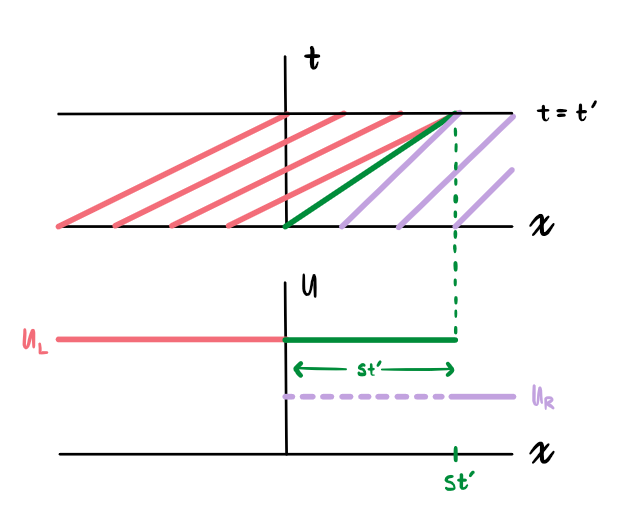
\includegraphics[width=1.0\textwidth]{riemann_shockwave.png}
        \caption{Resolution of a Riemann problem when $u_L > u_R > 0$. A shockwave propagates to the right with speed $(u_L+u_R)/2$.}
        \label{fig:shock}
    \end{subfigure}\hfill
    \begin{subfigure}{.48\textwidth}
        \centering
        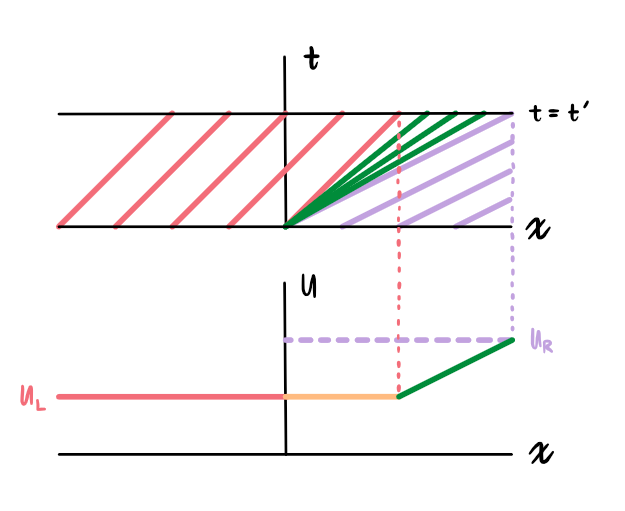
\includegraphics[width=1\textwidth]{riemann_rarefaction.png}
        \caption{Resolution of a Riemann problem when $0<u_L<u_R$. A rarefaction wave fills the void left by the characteristics.}
        \label{fig:rarefaction}
    \end{subfigure}
    \caption{Resolving the discontinuity in a Riemann problem.}
    \label{fig:riemann_discontinuities}
\end{figure}

\subsection{Convergence}



\subsection{High-Resolution Methods}

shit i dont fully understand how to implement

\section{Experiments}

We will be verifying our theory experimentally on five different problems. The first two are Riemann problems which are `easy' in the sense that a MATH student familiar with the relevant material should be able to characterize the solution completely. The consequence of this is that we can hard-code the solutions to compare against with respect to accuracy, both for our methods and for the Physics Informed Neural Network (PINN).

In contrast, we are unable to resolve the `hard' problems analytically and so cannot directly compute the accuracy of our methods. Instead, we will have to employ numerical convergence studies and rely on the soundness of the underlying theory.

\subsection{`Easy' Problems}

\subsubsection{Riemann problem: shockwave}

The initial value problem (IVP) of interest is
\begin{equation}\label{IVP:shock}
    \begin{cases}
        u_t + uu_x = 0 \quad x \in (-1,1), \: t > 0 \\
        u(-\pi,t) = 1 \\
        u(\pi,t) = 0 \\
        u(x,0) = u_0(x)
    \end{cases} 
\end{equation}
where 
\begin{equation}
    u_0(x) = \begin{cases}
        1 \qquad & x < 0 \\
        0 \qquad & x \geq 0
    \end{cases}
\end{equation}

Following our prior discussion, the analytical solution is characterized by a shockwave, and is given by
\begin{equation}
    u(x,t) = \begin{cases}
        1 \qquad & x < t/2 \\
        0 \qquad & x \geq t/2
    \end{cases}
\end{equation}

\subsubsection{Riemann problem: rarefaction wave}

We modify the \eqref{IVP:shock} slightly so that its solution exhibits a rarefaction fan
\begin{equation}\label{IVP:shock}
    \begin{cases}
        u_t + uu_x = 0 \quad x \in (-1,1), \: t > 0 \\
        u(-\pi,t) = 0 \\
        u(\pi,t) = 1 \\
        u(x,0) = u_0(x)
    \end{cases} 
\end{equation}
where 
\begin{equation}
    u_0(x) = \begin{cases}
        0 \qquad & x < 0 \\
        1 \qquad & x \geq 0
    \end{cases}
\end{equation}

Instead of a shockwave, the analytical solution is characterized by a rarefaction wave, and is given by
\begin{equation}
    u(x,t) = \begin{cases}
        0 \qquad & x < 0 \\
        x/t \qquad & 0 \leq x \leq t \\
        1 \qquad & x > t
    \end{cases}
\end{equation}

\begin{comment}
\begin{itemize}
	\item \textbf{Riemann Problem}
	
	The Riemann Problem studies the formation of shocks. The initial condition is as follows
	\begin{equation}
		u(x,0) = 
	    \begin{cases}
	      	u_L & \text{if } x < 0 \\
			u_R & \text{if } x \geq 0
	    \end{cases}
	\end{equation}
	where $u_L > u_R$. In our experiment, we set $u_L = 1$ and $u_R = 0$. The true solution is
	\begin{equation}
		u(x,t) = 
	    \begin{cases}
	      	u_L = 1 & \text{if } x < st \\
			u_R = 0 & \text{if } x \geq st
	    \end{cases}
	\end{equation}
	where \[s = \frac{u_L + u_R}{2}\ = \frac{1}{2}\] is the speed of the shock. This is known as the Rankine-Hugoniot condition. In our experiment, we shifted right spacially by $\pi$ and used the boundaries $[0, 2\pi]$. This made our plots more consistent with the harder problems, which are all $[0, 2\pi]$ periodic.
	
	RESULTSSSSSSSSSSSSSSSS
	
	\item \textbf{Rarefaction Wave}
	
	If we take the Riemann Problem but instead have $u_L < u_R$, a shock will not form. In this case we get what is called a rarefaction wave. In our experiment, we set $u_L = 0$ and $u_R = 1$. The true solution is
	\begin{equation}
		u(x,t) = 
	    \begin{cases}
	      	u_L = 0 & \text{if } x \leq {u_L}t \\
			\frac{x}{t} & \text{if } {u_L}t < x < {u_R}t \\
			u_R = 1 & \text{if } x \geq {u_R}t
	    \end{cases}
	\end{equation}
	
\end{itemize}
\end{comment}

\subsection{`Hard' Problems}

\subsubsection{Square wave}

Our first IVP has the form
\begin{equation}
    \begin{cases}
        u_t + uu_x = 0, \quad x \in [0, 2\pi], \: t>0 \\
        u(x,0) = u_0(x) \\
        u(0,t) = u(2\pi,t), \quad t > 0
    \end{cases}
\end{equation}
where
\begin{equation}
    u_0(x) = 
    \begin{cases}
        1 \qquad &  x \in [\pi/2, 3\pi/2] \\
        0 \qquad & \text{otherwise} 
    \end{cases}
\end{equation}

\subsubsection{Sine wave}

The IVP is given by
\begin{equation}
    \begin{cases}
        u_t + uu_x = 0, \quad x \in [0, 2\pi], \: t>0 \\
        u(x,0) = \sin(x) \\
        u(0,t) = u(2\pi,t), \quad t > 0
    \end{cases}
\end{equation}

\subsubsection{Sine-squared wave}

We modify the prior IVP slightly
\begin{equation}
    \begin{cases}
        u_t + uu_x = 0, \quad x \in [0, 2\pi], \: t>0 \\
        u(x,0) = \sin^2(x) \\
        u(0,t) = u(2\pi,t), \quad t > 0
    \end{cases}
\end{equation}

\begin{comment}
\begin{itemize}
	\item \textbf{Sinusoidal Initial Conditions}
	
	We experimented with the following IVP
	\begin{equation}
	    \begin{cases}
	      	u_t + uu_x = 0, \: x \in [0, 2\pi], \: t>0 \\
			u(x,0) = sin(x) \\
			u(0,t) = u(2\pi,t) \: \forall t
	    \end{cases}
	\end{equation}
	
	\item \textbf{Squared Sinusoidal Initial Conditions}
	
	We experimented with the following IVP
	\begin{equation}
	    \begin{cases}
	      	u_t + uu_x = 0, \: x \in [0, 2\pi], \: t>0 \\
			u(x,0) = sin^2(\frac{x}{2}) \\
			u(0,t) = u(2\pi,t) \: \forall t
	    \end{cases}
	\end{equation}
	
	\item \textbf{Squared Sinusoidal Initial Conditions}
	
	We experimented with the following IVP
	\begin{equation}
	    \begin{cases}
	      	u_t + uu_x = 0, \: x \in [0, 2\pi], \: t>0 \\
			u(x,0) = g(x) \\
			u(0,t) = u(2\pi,t) \: \forall t
	    \end{cases}
	\end{equation}
	where
	\begin{equation}
		g(x) = 
	    \begin{cases}
	      	1 & \text{if } x \in [\frac{\pi}{2}, \frac{3\pi}{2}] \\
			0 & \text{otherwise} 
	    \end{cases}
	\end{equation}
		
\end{itemize}
\end{comment}

\section{Conclusion}

this shit was way harder than i thought it would be

\newpage
\appendix
\section{Appendix}
\subsection{Code}

All project code can be found on our GitHub page: \url{https://github.com/agormann/MACM416-project}. As a courtesy, we have also included our code in this document, below.

[insert code]

\subsection{Analytical Solution via the Method of Characteristics}

We wish to solve the 1-D inviscid Burgers' equation analytically.

Given data on some curve $ \Gamma \subset \overline{\Omega} $, we are looking specific parametric curves $ (x(t), t) $ which connect points $(x, t) \in \Omega$ to $ \Gamma $. We want these curves to be precisely those which are parallel to the vector $(u, 1)$, that is
\[
    \frac{dx}{dt} = \frac{u(x(t), t)}{1} = u(x(t), t)
\]

Now supposing that $u$ solves (2), let $z(t)$ denote the value of $u$ along a characteristic, i.e. 
\[
    z(t) = u(x(t), t)
\]
Then by the chain rule
\[
    \frac{dz}{dt} = \partial_x u(x(t), t) \frac{dx}{dt}u(x(t), t) + \partial_t u(x(t), t)
\]
but $ x'(t) = u(x,t) $, so
\[
    \frac{dz}{dt} = \partial_t u(x(t), t) + u(x,t)\partial_x u(x(t), t)
\]
which is precisely 0 by (2). Hence, we have the following coupled system of ODEs
\begin{equation}
    \begin{cases}
        x'(t) = z(t) = u(x(t), t) \\
        z'(t) = 0
    \end{cases}
\end{equation}
Integrating the second term, we get that
\[
    z(t) = z_0
\]
for some $ z_0 \in \R $. But $z(t) = u(x(t), t)$, so then $u(x(t), t) = z_0$. This corroborates our findings with (3). Now by integrating the first term, we get
\begin{equation}
    x(t) = z_0t + x_0
\end{equation}
where $ x_0 \in \R $. Evaluating at $t=0$, we have that $x(0) = x_0$. Now assuming we are prescribed some initial condition $u(x,0) = g(x)$, we have that (5) becomes
\begin{equation}
    x(t) = g(x_0)t + x_0
\end{equation}
which are exactly those characteristic curves we initially sought.

% bibliography
\nocite{choksi2022}
\nocite{iserles2009}
% \nocite{kutz2013}
% \nocite{trefethen2001}
% \nocite{learncfd}
% \nocite{evans2010}
\nocite{leveque1992}
\nocite{leveque2002}
\printbibliography

\end{document}